\section{x86: \RU{3 аргумента}\EN{3 arguments}}

\subsection{MSVC}

\RU{Компилируем при помощи MSVC 2010 Express, и в итоге получим:}
\EN{Let's compile it by MSVC 2010 Express and we got:}

\begin{lstlisting}
$SG3830	DB	'a=%d; b=%d; c=%d', 00H

...

	push	3
	push	2
	push	1
	push	OFFSET $SG3830
	call	_printf
	add	esp, 16					; 00000010H
\end{lstlisting}

\RU{Все почти то же, за исключением того, что теперь видно, что аргументы для \printf заталкиваются в стек в обратном порядке: самый первый аргумент заталкивается последним.}
\EN{Almost the same, but now we can see the \printf arguments are pushed onto the stack in reverse order. The first argument is pushed last.}

\RU{Кстати, вспомним что переменные типа \Tint в 32-битной системе, как известно, имеет ширину 32 бита, это 4 байта}
\EN{By the way, variables of \Tint type in 32-bit environment have 32-bit width, that is 4 bytes}.

\RU{Итак, у нас всего 4 аргумента. $4*4 = 16$ ~--- именно 16 байт занимают в стеке указатель на строку плюс еще 3 числа типа \Tint.}
\EN{So, we have here 4 arguments. $4*4 = 16$~---they occupy exactly 16 bytes in the stack: a 32-bit pointer to a string and 3 numbers of type \Tint.}

\index{x86!\Instructions!ADD}
\index{x86!\Registers!ESP}
\index{cdecl}
\RU{Когда при помощи инструкции \TT{``ADD ESP, X''} корректируется \glslink{stack pointer}{указатель стека} \ESP 
после вызова какой-либо функции, зачастую можно сделать вывод о том, сколько аргументов 
у вызываемой функции было, разделив X на 4.}
\EN{When the \gls{stack pointer} (\ESP register) is corrected by \TT{``ADD ESP, X''}
instruction after a function 
call, often, the number of function arguments can be deduced here: just divide X by 4.}

\RU{Конечно, это относится только к cdecl-методу передачи аргументов через стек.}
\EN{Of course, this is related only to \IT{cdecl} calling convention.}

\RU{См. также в соответствующем разделе о способах передачи аргументов через стек}
\EN{See also the section about calling conventions}~(\ref{sec:callingconventions}).

\RU{Иногда бывает так, что подряд идут несколько вызовов разных функций, 
но стек корректируется только один раз, после последнего вызова:}
\EN{It is also possible for the compiler to merge several \TT{``ADD ESP, X''} instructions into one, after the last call:}

\begin{lstlisting}
push a1
push a2
call ...
...
push a1
call ...
...
push a1
push a2
push a3
call ...
add esp, 24
\end{lstlisting}

\subsection{MSVC \AndENRU \olly}
\index{\olly}

\RU{Попробуем этот же пример в}\EN{Now let's try to load this example in} \olly.
\RU{Это один из наиболее популярных win32-отладчиков user-режима}\EN{It is one of the most 
popular user-land win32 debugger}.
\RU{Мы можем компилировать наш пример в}\EN{We can try to compile our example in} MSVC 2012 
\RU{с опцией}\EN{with} \TT{/MD} \RU{что означает, линковать с библиотекой}\EN{option, meaning, to link 
against} \TT{MSVCR*.DLL},
\RU{чтобы импортируемые ф-ции были хорошо видны в отладчике}\EN{so we will able to see imported 
functions clearly in debugger}.

\RU{Затем загружаем исполняемый файл в}\EN{Then load executable in} \olly.
\RU{Самый первый брякпойнт в}\EN{The very first breakpoint is in} \TT{ntdll.dll}, \RU{нажмите}\EN{press} 
F9 (\RU{запустить}\EN{run}).
\RU{Второй брякпойнт в}\EN{The second breakpoint is in} \ac{CRT}-\RU{коде}\EN{code}.
\RU{Теперь мы должны найти ф-цию}\EN{Now we should find} \main\EN{ function}.

\RU{Найдите этот код скроллируя окно кода до самого верха (MSVC располагает ф-цию \main в самом начале
секции кода)}\EN{Find this code by scrolling the code to the very bottom (MSVC allocates \main function at
the very beginning of the code section)}: 
\figref{fig:printf3_olly_1}.\\
\\
\RU{Кликните на инструкции}\EN{Click on} \TT{PUSH EBP}\RU{, нажмите}\EN{ instruction, press} F2 
(\RU{установка брякпойнта}\EN{set breakpoint}) \RU{и нажмите}\EN{and press} F9 (\RU{запустить}\EN{run}).
\RU{Нам нужно произвести все эти манипуляции, чтобы пропустить \ac{CRT}-код, потому что нам он пока
не интересен}\EN{We need to do these manupulations in order to skip \ac{CRT}-code, because, we don't really 
interesting in it yet}.\\
\\
\RU{Нажмите}\EN{Press} F8 (\stepover) 6 \RU{раз, т.е., пропустить
6 инструкций}\EN{times, i.e., skip 6 instructions}: \figref{fig:printf3_olly_2}.\\
\\
\RU{Теперь}\EN{Now the} \ac{PC} \RU{указывает на инструкцию}\EN{points to the}
\TT{CALL printf}\EN{ instruction}.
\olly, \RU{как и другие отладчики, подсвечивает регистры со значениями, которые изменились}
\EN{like other debuggers, highlights value of registers which were changed}.
\RU{Так что, каждый раз, когда мы нажимаем}\EN{So each time you press F8}, \EIP 
\RU{изменяется и его значение подсвечивается красным}\EN{is changing and its value looking red}.
\ESP \RU{также меняется, потому что значения заталкиваются в стек}\EN{is changing as well, 
because values are pushed into the stack}.\\
\\
\RU{Где находятся эти значения в стеке}\EN{Where are the values in the stack}?
\RU{Посмотрите на правое/нижнее окно в отладчике}\EN{Take a look into right/bottom window of debugger}:

\begin{figure}[H]
\centering
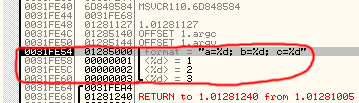
\includegraphics[scale=0.66]{patterns/03_printf/olly3_stack.png}
\caption{\olly: \RU{стек, после того как значения там сохранены}\EN{stack after values pushed}
(\RU{я сделал здесь округлую красную пометку в графическом редакторе}\EN{I made round red mark 
here in graphics editor})}
\end{figure}

\RU{Так что здесь видно 3 столбца: адрес в стеке, значение в стеке и еще дополнительный комментарий
от \olly}\EN{So we can see there 3 columns: address in the stack, 
value in the stack and some additional \olly comments}. 
\olly \RU{понимает}\EN{understands} \printf\RU{-строки}\EN{-like strings}, 
\RU{так что он показывает здесь и строку и 3 значения \IT{привязанных} к ней}\EN{so it reports the 
string here and 3 values \IT{attached} to it}.

\RU{Можно кликнуть правой кнопкой мыши на строке формата, кликнуть на ``Follow in dump''
и строка формата появится в окне слева внизу, где всегда виден какой-либо участок памяти}
\EN{It is possible to right-click on the format string, click on ``Follow in dump'',
and the format string will appear in the window at the left-bottom part, where some memory part
is always seen}.
\RU{Эти значения в памяти можно редактировать}\EN{These memory values can be edited}.
\RU{Можно изменить саму строку формата, и тогда результат работы нашего примера будет другой}
\EN{It is possible to change the format string, and then the result of our example will be different}.
\RU{В данном случае, пользы от этого немного, но для упражнения это полезно,
чтобы начать чувствовать как тут всё работает}\EN{It is probably not very useful now, but it's very
good idea for doing it as exercise, to get feeling how everything is works here}.

\RU{Нажмите}\EN{Press} F8 (\stepover).

\RU{В консоли мы видим вывод}\EN{In the console we'll see the output}:

\begin{figure}[H]
\centering
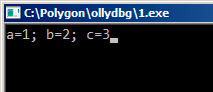
\includegraphics[scale=0.66]{patterns/03_printf/olly3_console.png}
\caption{\RU{Ф-ция }\printf \RU{исполнилась}\EN{function executed}}
\end{figure}

\RU{Посмотрим, как изменились регистры и состояние стека}\EN{Let's see how registers and stack state 
are changed}: \figref{fig:printf3_olly_3}.

\RU{Регистр }\EAX \RU{теперь содержит}\EN{register now contains} \TT{0xD} (13).
That's correct, \printf returns number of characters printed.
\RU{Значение }\EIP \RU{изменилось: действительно, теперь здесь адрес инструкции после}
\EN{value is changed: indeed, now there is address of the instruction after} \TT{CALL printf}.
\RU{Значения регистров }\ECX \AndENRU \EDX \RU{также изменились}\EN{values are changed as well}.
\RU{Очевидно, внутренности ф-ции \printf используют их для каких-то своих нужд}\EN{Apparently, 
\printf function's hidden machinery used them for its own needs}.

\RU{Очень важный момент в том что значение \ESP не изменилось. И состояние стека также!}
\EN{A very important thing is that \ESP value is not changed. And stack state too!}
\RU{Мы ясно видим здесь и строку формата и соответствующие ей 3 значения, они все еще здесь}
\EN{We clearly see that format string and corresponding 3 values are still there}.
\RU{Действительно, по соглашению вызовов \IT{cdecl}, вызывающая ф-ция не очищает аргументы из стека}
\EN{Indeed, that's \IT{cdecl} calling convention, calling function doesn't clear arguments in stack}.
\RU{Это должна делать вызывающая ф-ция}\EN{It's caller's duty to do so}.

\RU{Нажмите}\EN{Press} F8 \RU{снова, чтобы исполнилась инструкция}\EN{again to execute} 
\TT{ADD ESP, 10}\EN{ instruction}: \figref{fig:printf3_olly_4}.

\ESP \RU{изменился, но значения все еще в стеке}\EN{is changed, but values are still in the stack}!
\RU{Конечно, никому не нужно заполнять эти значения нулями или что-то в этом роде}\EN{Yes, 
of course, no one needs to fill these values by zero or something like that}.
\RU{Потому что всё что выше указателя стека}\EN{Because, everything above stack pointer} (\ac{SP}) 
\RU{это}\EN{is} \IT{\RU{шум}\EN{noise}} \OrENRU \IT{\RU{мусор}\EN{garbage}}, \RU{это всё не имеет
особой ценности}\EN{it has no value at all}.
\RU{Было бы очень затратно по времени очищать ненужные элементы стека, к тому же, никому это и не 
нужно}\EN{It would be time consuming to clear unused stack entries, besides, no one really needs to}.

\begin{figure}[H]
\centering
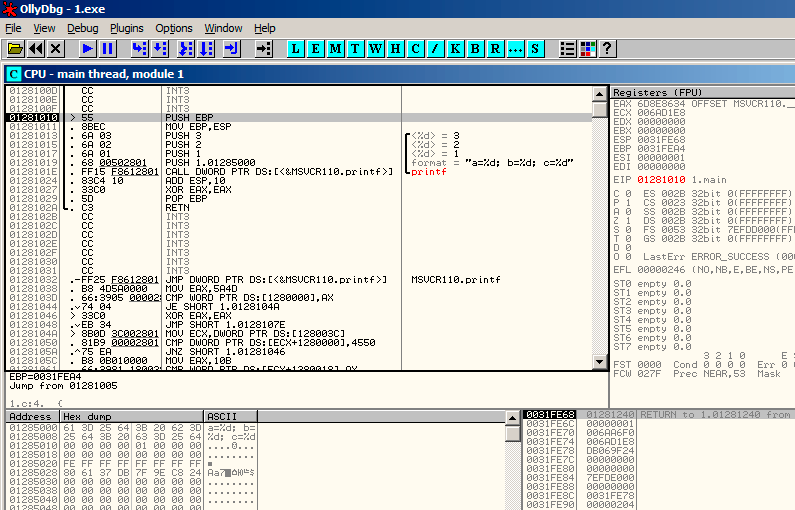
\includegraphics[scale=\FigScale]{patterns/03_printf/olly3_1.png}
\caption{\olly: \RU{самое начало ф-ции}\EN{the very start of the} \main\EN{ function}}
\label{fig:printf3_olly_1}
\end{figure}

\begin{figure}[H]
\centering
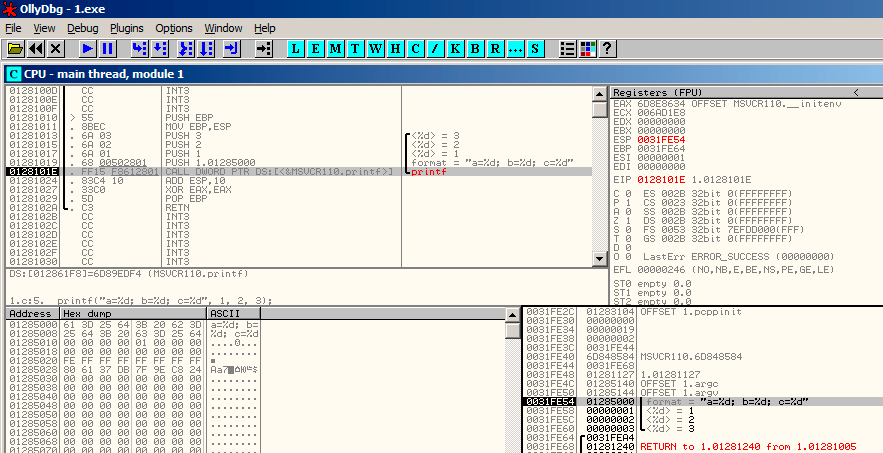
\includegraphics[scale=\FigScale]{patterns/03_printf/olly3_2.png}
\caption{\olly: \RU{перед исполнением}\EN{before} \printf\EN{ execution}}
\label{fig:printf3_olly_2}
\end{figure}

\begin{figure}[H]
\centering
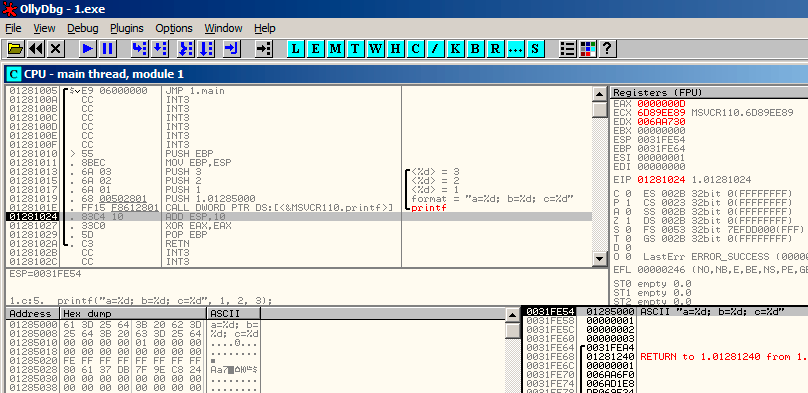
\includegraphics[scale=\FigScale]{patterns/03_printf/olly3_3.png}
\caption{\olly: \RU{после исполнения}\EN{after} \printf\EN{ execution}}
\label{fig:printf3_olly_3}
\end{figure}

\begin{figure}[H]
\centering
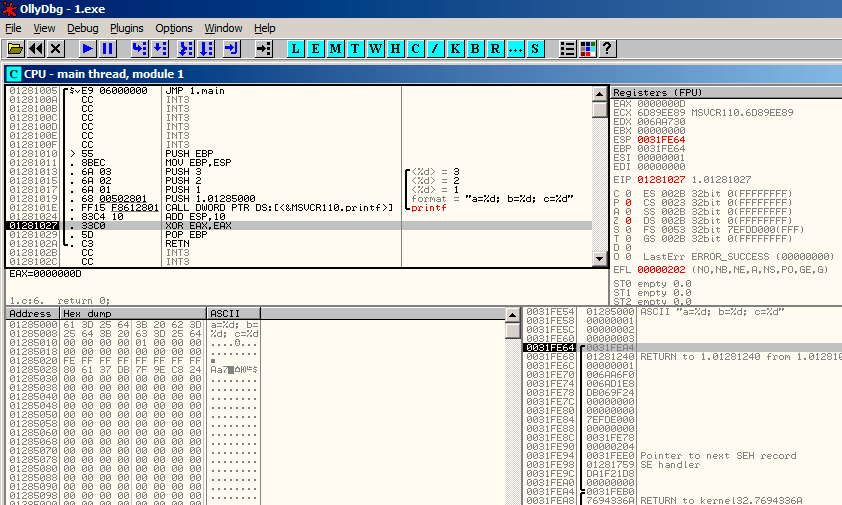
\includegraphics[scale=\FigScale]{patterns/03_printf/olly3_4.png}
\caption{\olly: \RU{после исполнения инструкции}\EN{after} \TT{ADD ESP, 10}\EN{ instruction execution}}
\label{fig:printf3_olly_4}
\end{figure}

\subsection{GCC}

\RU{Скомпилируем то же самое в Linux при помощи GCC 4.4.1 и посмотрим в \IDA что вышло:}
\EN{Now let's compile the same program in Linux using GCC 4.4.1 and take a look in \IDA what we got:}

\begin{lstlisting}
main            proc near

var_10          = dword ptr -10h
var_C           = dword ptr -0Ch
var_8           = dword ptr -8
var_4           = dword ptr -4

                push    ebp
                mov     ebp, esp
                and     esp, 0FFFFFFF0h
                sub     esp, 10h
                mov     eax, offset aADBDCD ; "a=%d; b=%d; c=%d"
                mov     [esp+10h+var_4], 3
                mov     [esp+10h+var_8], 2
                mov     [esp+10h+var_C], 1
                mov     [esp+10h+var_10], eax
                call    _printf
                mov     eax, 0
                leave
                retn
main            endp
\end{lstlisting}

\RU{Можно сказать, что этот короткий код, созданный GCC, отличается от кода MSVC только способом помещения 
значений в стек.
Здесь GCC снова работает со стеком напрямую без \PUSH/\POP.}
\EN{It can be said that the difference between code from MSVC and code from GCC is only in the method of placing arguments on the stack.
Here GCC is working directly with the stack without \PUSH/\POP.}

\subsection{GCC \AndENRU GDB}
\index{GDB}

\RU{Попробуем также этот пример и в \ac{GDB} в Linux}\EN{Let's try this example also in \ac{GDB} in Linux}.

\TT{-g} \RU{означает генерировать отладочную информацию в выходном исполняемом файле}\EN{mean produce 
debug information into executable file}.

\begin{lstlisting}
$ gcc 1.c -g -o 1
\end{lstlisting}

\begin{lstlisting}
$ gdb 1
GNU gdb (GDB) 7.6.1-ubuntu
Copyright (C) 2013 Free Software Foundation, Inc.
License GPLv3+: GNU GPL version 3 or later <http://gnu.org/licenses/gpl.html>
This is free software: you are free to change and redistribute it.
There is NO WARRANTY, to the extent permitted by law.  Type "show copying"
and "show warranty" for details.
This GDB was configured as "i686-linux-gnu".
For bug reporting instructions, please see:
<http://www.gnu.org/software/gdb/bugs/>...
Reading symbols from /home/dennis/polygon/1...done.
\end{lstlisting}

\begin{lstlisting}[caption=\RU{установим брякпойнт на}\EN{let's set breakpoint on} \printf]
(gdb) b printf
Breakpoint 1 at 0x80482f0
\end{lstlisting}

\RU{Запукаем}\EN{Run}.
\RU{Здесь у нас нет исходного кода ф-ции}\EN{There are no} \printf 
\RU{так что \ac{GDB} не может показать его исходный код, но могла бы}\EN{function source code here, 
so \ac{GDB} can't show its source, but may do so}.

\begin{lstlisting}
(gdb) run
Starting program: /home/dennis/polygon/1 

Breakpoint 1, __printf (format=0x80484f0 "a=%d; b=%d; c=%d") at printf.c:29
29	printf.c: No such file or directory.
\end{lstlisting}

\RU{Выдать 10 элементов стека. Левый столбец это адрес в стеке.}
\EN{Print 10 stack elements. Left column is an address in stack.}

\begin{lstlisting}
(gdb) x/10w $esp
0xbffff11c:	0x0804844a	0x080484f0	0x00000001	0x00000002
0xbffff12c:	0x00000003	0x08048460	0x00000000	0x00000000
0xbffff13c:	0xb7e29905	0x00000001
\end{lstlisting}

\RU{Самый первый элемент это}\EN{The very first element is} \ac{RA} (\TT{0x0804844a}).
\RU{Мы можем удостовериться в этом, дизассемблируя память по этому адресу}\EN{We can be sure 
in it by disassembling the memory at this address}:

\begin{lstlisting}
(gdb) x/5i 0x0804844a
   0x804844a <main+45>:	mov    $0x0,%eax
   0x804844f <main+50>:	leave  
   0x8048450 <main+51>:	ret    
   0x8048451:	xchg   %ax,%ax
   0x8048453:	xchg   %ax,%ax
\end{lstlisting}

\RU{Две инструкции}\EN{Two} \TT{XCHG} 
\RU{это, вероятно, какой-то случайный мусор, который мы пока что можем игнорировать}
\EN{instructions, apparently, is some random garbage, which we can ignore so far}.

\RU{Второй элемент}\EN{The second element} (\TT{0x080484f0}) \RU{это адрес
строки формата}\EN{is an address of format string}:

\begin{lstlisting}
(gdb) x/s 0x080484f0
0x80484f0:	"a=%d; b=%d; c=%d"
\end{lstlisting}

\RU{Остальные 3 элемента}\EN{Other 3 elements} (1, 2, 3) \RU{это аргументы ф-ции}\EN{are} 
\printf\EN{ arguments}.
\RU{Остальные элементы это может быть и мусор в стеке, но могут быть и значения
от других ф-ций, их локальные переменные, итд}\EN{Other elements may be just ``garbage'' present in stack,
but also may be values from other functions, their local variables, etc}.
\RU{Пока что мы можем игнорировать их}\EN{We can ignore it yet}.

\RU{Исполняем}\EN{Execute} ``finish''. 
\RU{Это значит, исполнять до конца ф-ции}\EN{This mean, execute till function end}. 
\RU{Здесь это означает: исполнять до завершения}\EN{Here it means: execute till the finish of} \printf.

\begin{lstlisting}
(gdb) finish
Run till exit from #0  __printf (format=0x80484f0 "a=%d; b=%d; c=%d") at printf.c:29
main () at 1.c:6
6		return 0;
Value returned is $2 = 13
\end{lstlisting}

\ac{GDB} \RU{показывает, что вернула}\EN{shows what} \printf \RU{в}\EN{returned in} \EAX (13).
\RU{Это, так же как и в примере с \olly, количество напечатанных символов}
\EN{This is number of characters printed, just like in the example with \olly}.

\RU{А еще мы видим}\EN{We also see} ``return 0;'' \RU{и что это выражение находится в файле 
\TT{1.c} в строке 6}\EN{and the information that this expression is in the \TT{1.c} file at the line 6}.
\RU{Действительно, файл \TT{1.c} лежит в текущем директории и \ac{GDB} находит там эту строку}
\EN{Indeed, the \TT{1.c} file is located in the current directory, and \ac{GDB} finds the string there}.
\RU{Как \ac{GDB} знает, какая строка Си-кода сейчас исполняется}\EN{How \ac{GDB} knows, which C-code line
is being executed now}?
\RU{Это связано с тем фактом, что компилятор, генерируя отладочную информацию,
также сохраняет информацию о 
соответствии строк в исходном коде и адресов инструкций}\EN{This is related to the fact that compiler,
while generating debugging information, also saves a table of relations between source code line
numbers and instruction addresses}.
GDB \RU{это всё-таки отладчик уровня исходных текстов}\EN{is source-level debugger, after all}.

\RU{Посмотрим регистры}\EN{Let's examine registers}.
13 \InENRU \EAX:

\begin{lstlisting}
(gdb) info registers
eax            0xd	13
ecx            0x0	0
edx            0x0	0
ebx            0xb7fc0000	-1208221696
esp            0xbffff120	0xbffff120
ebp            0xbffff138	0xbffff138
esi            0x0	0
edi            0x0	0
eip            0x804844a	0x804844a <main+45>
...
\end{lstlisting}

\RU{Попробуем дизассемблировать текущие инструкции}\EN{Let's disassemble current instructions}.
\RU{Стрелка указывает на инструкцию, которая будет исполнена следующей}\EN{Arrow points to the 
instruction being executed next}.

\begin{lstlisting}
(gdb) disas
Dump of assembler code for function main:
   0x0804841d <+0>:	push   %ebp
   0x0804841e <+1>:	mov    %esp,%ebp
   0x08048420 <+3>:	and    $0xfffffff0,%esp
   0x08048423 <+6>:	sub    $0x10,%esp
   0x08048426 <+9>:	movl   $0x3,0xc(%esp)
   0x0804842e <+17>:	movl   $0x2,0x8(%esp)
   0x08048436 <+25>:	movl   $0x1,0x4(%esp)
   0x0804843e <+33>:	movl   $0x80484f0,(%esp)
   0x08048445 <+40>:	call   0x80482f0 <printf@plt>
=> 0x0804844a <+45>:	mov    $0x0,%eax
   0x0804844f <+50>:	leave  
   0x08048450 <+51>:	ret    
End of assembler dump.
\end{lstlisting}

\ac{GDB} \RU{показывает дизассемблированный листинг в формате}\EN{shows disassembly in} AT\&T 
\RU{по умолчанию}\EN{syntax by default}.
\RU{Но можно также переключиться в формат Intel}\EN{It's possible to switch to Intel syntax}:

\begin{lstlisting}
(gdb) set disassembly-flavor intel
(gdb) disas
Dump of assembler code for function main:
   0x0804841d <+0>:	push   ebp
   0x0804841e <+1>:	mov    ebp,esp
   0x08048420 <+3>:	and    esp,0xfffffff0
   0x08048423 <+6>:	sub    esp,0x10
   0x08048426 <+9>:	mov    DWORD PTR [esp+0xc],0x3
   0x0804842e <+17>:	mov    DWORD PTR [esp+0x8],0x2
   0x08048436 <+25>:	mov    DWORD PTR [esp+0x4],0x1
   0x0804843e <+33>:	mov    DWORD PTR [esp],0x80484f0
   0x08048445 <+40>:	call   0x80482f0 <printf@plt>
=> 0x0804844a <+45>:	mov    eax,0x0
   0x0804844f <+50>:	leave  
   0x08048450 <+51>:	ret    
End of assembler dump.
\end{lstlisting}

\RU{Исполняем следующую инструкцию}\EN{Execute next instruction}.
\ac{GDB} \RU{покажет закрывающуюся скобку, означая, что это конец блока в ф-ции}\EN{shows ending bracket, 
meaning, this is ending block of function}.

\begin{lstlisting}
(gdb) step
7	};
\end{lstlisting}

\RU{Посмотрим регистры после исполнения инструкции}\EN{Let's see registers after} 
\TT{MOV EAX, 0}\EN{ instruction execution}.
\EAX \RU{здесь уже действительно ноль}\EN{here is zero indeed}.

\begin{lstlisting}
(gdb) info registers
eax            0x0	0
ecx            0x0	0
edx            0x0	0
ebx            0xb7fc0000	-1208221696
esp            0xbffff120	0xbffff120
ebp            0xbffff138	0xbffff138
esi            0x0	0
edi            0x0	0
eip            0x804844f	0x804844f <main+50>
...
\end{lstlisting}
